\section*{Introduction}

A distributed system is made highly available when individual servers are
allowed to operate independently without coordination that may be prone to
failure or high latency.
The independent nature of the server's behavior means that it can immediately
respond to client requests, but that it does so from a limited, local
perspective which may be inconsistent with another server's response.
If individual servers in a system were allowed to remain wholly independent,
individual requests from clients to different servers would create a lack of
order or predictability, a gradual decline into inconsistency, e.g. the
system would experience \textit{entropy}.
To combat the effect of entropy while still remaining highly available,
servers engage in \textit{anti-entropy sessions}~\cite{terry_session_1994} at
a routine interval, a process that occurs in the background of client
requests.

Anti-entropy sessions synchronize the state between servers ensuring that,
at least briefly, the local state is consistent with a portion of the global
state of the system.
If all servers engage in anti-entropy sessions, the system is able to make
some reasonable guarantees about the timeliness of responses; the most famous
of which is that in the absence of requests the system will become
consistent, eventually.
More specifically, inconsistencies in the form of stale reads can be bound by
likelihoods that are informed by the latency of anti-entropy sessions and the
size of the system~\cite{bailis_quantifying_2014}.
Said another way, overall consistency is improved in an eventually consistent
system by decreasing the likelihood of a stale read, which is tuned by
improving the \textit{visibility latency} of a write, the speed at which a
write is propagated to a significant portion of servers.
This idea has led many system designers to decide that ``eventual consistency
is consistent enough''~\cite{bermbach_eventual_2011,wada2011data}
particularly in a data center context where visibility latency is far below
the rate of client requests, leading to practically strong consistency.

Recently there have been two important changes in considerations for the
design of such systems that have led us to reevaluate propagation speed:
systems are getting larger and are becoming geographically distributed
outside of the datacenter.
Scaling an eventually consistent system to dozens or even hundreds of nodes
increases the radius of the network, which leads to increased noise during
anti-entropy; e.g. the possibility that an anti-entropy session will be
between two already synchronized nodes.
Geographic distribution and extra-datacenter networks increase the latency of
anti-entropy sessions so that inconsistencies become more apparent.
Large, geographically distributed systems are becoming the norm -- from
content delivery systems that span the globe, to mobile applications, to
future systems such a automated vehicular networks, and all will require
additional consistency guarantees without sacrificing availability.

We propose a new class of adaptive distributed data systems whose replicas
monitor their environment and modify their behavior to optimize consistency.
Anti-entropy utilizes gossip and rumor spreading to efficiently propagate
updates in a deterministic fashion without saturating the
network~\cite{haeupler_simple_2015,karp_randomized_2000,moreno_dynamics_2004}.
These protocols utilize uniform random selection of peers to synchronize
with, which means that a write occurring at one replica is not efficiently
propagated across the network.
We propose the use of \textit{multi-armed bandit}
algorithms~\cite{langford_epoch-greedy_2008,luo_efficient_2017} to modify the
probability of peer selection in order to optimize for fast, successful
synchronizations.
The result is a network topology that emerges according to access patterns
and network latency, often localizing replicas to produce efficient
synchronization, efficiency which lowers visibility latency and increases
consistency.

\section*{System Description}

A basic sketch of an eventually consistent system is as follows:

\section*{Bandit Approaches}

\begin{table}[]
\centering
\begin{tabular}{@{}|l|l|l|l|@{}}
\toprule
 & \textbf{Pull} & \textbf{Push} & \textbf{Total} \\ \midrule
Synchronize at least 1 object & 0.25 & 0.25 & 0.50 \\ \midrule
Synchronize multiple objects & 0.05 & 0.05 & 0.10 \\ \midrule
Latency <= 5ms (local) & 0.10 & 0.10 & 0.20 \\ \midrule
Latency <= 100ms (regional) & 0.10 & 0.10 & 0.20 \\ \midrule
\textit{Total} & \textit{0.50} & \textit{0.50} & \textit{1.00} \\ \bottomrule
\end{tabular}
\caption{Reward Function}
\label{tab:rewards}
\end{table}

\section*{Experiments}

\begin{figure}[t]
    \centering
    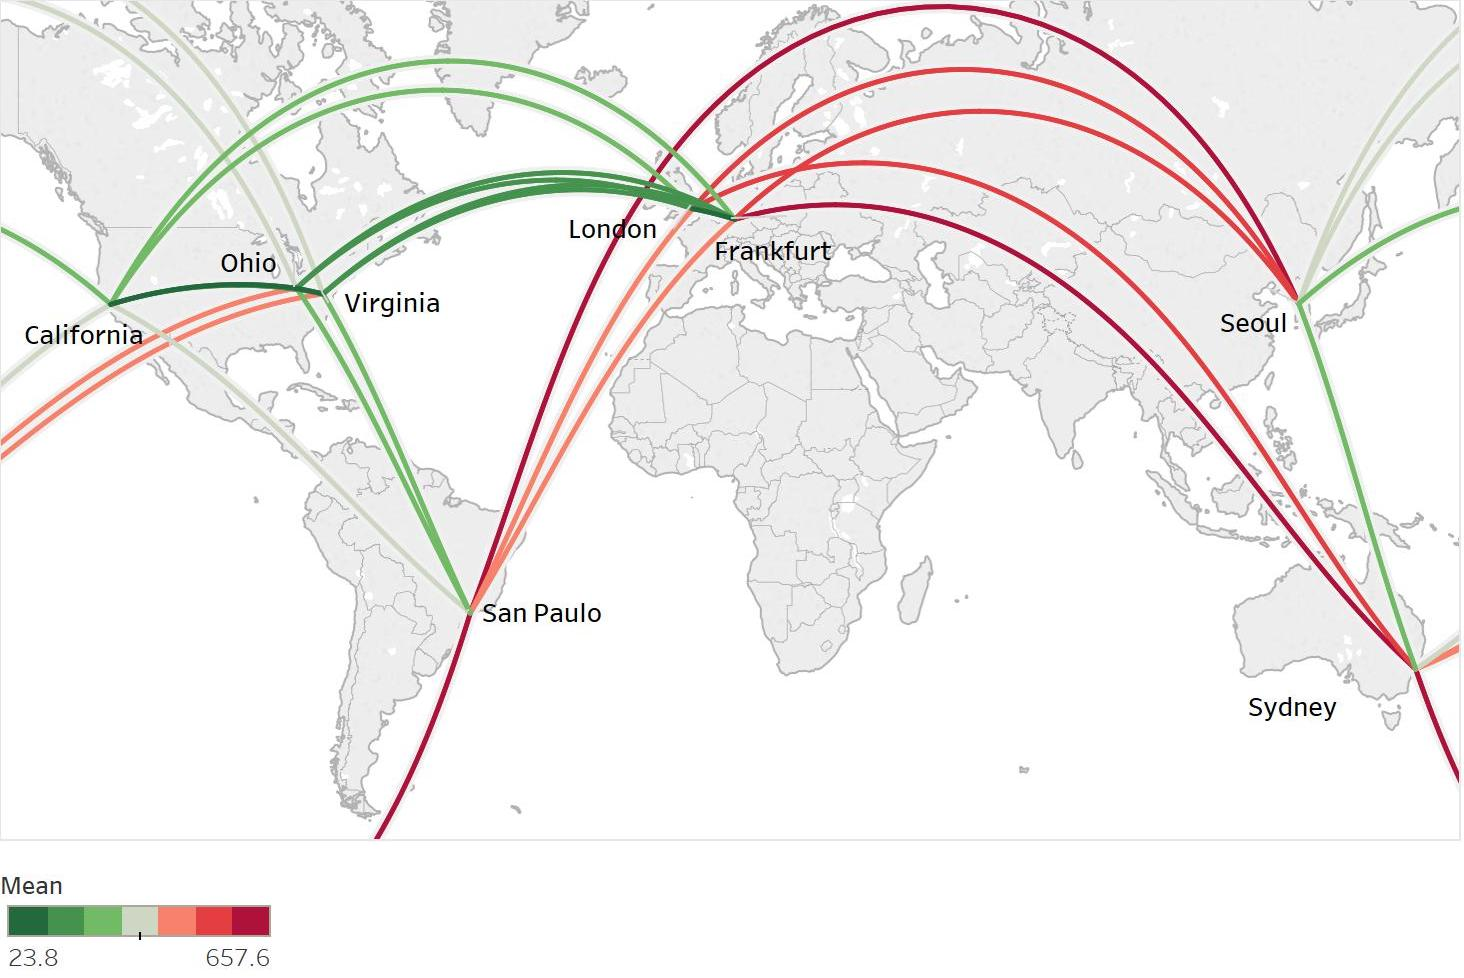
\includegraphics[width=0.5\textwidth]{figures/network}
    \caption{Geographically distributed network}
    \label{fig:network}
\end{figure}

\begin{figure*}[t]
    \centering
    \minipage{0.5\textwidth}
      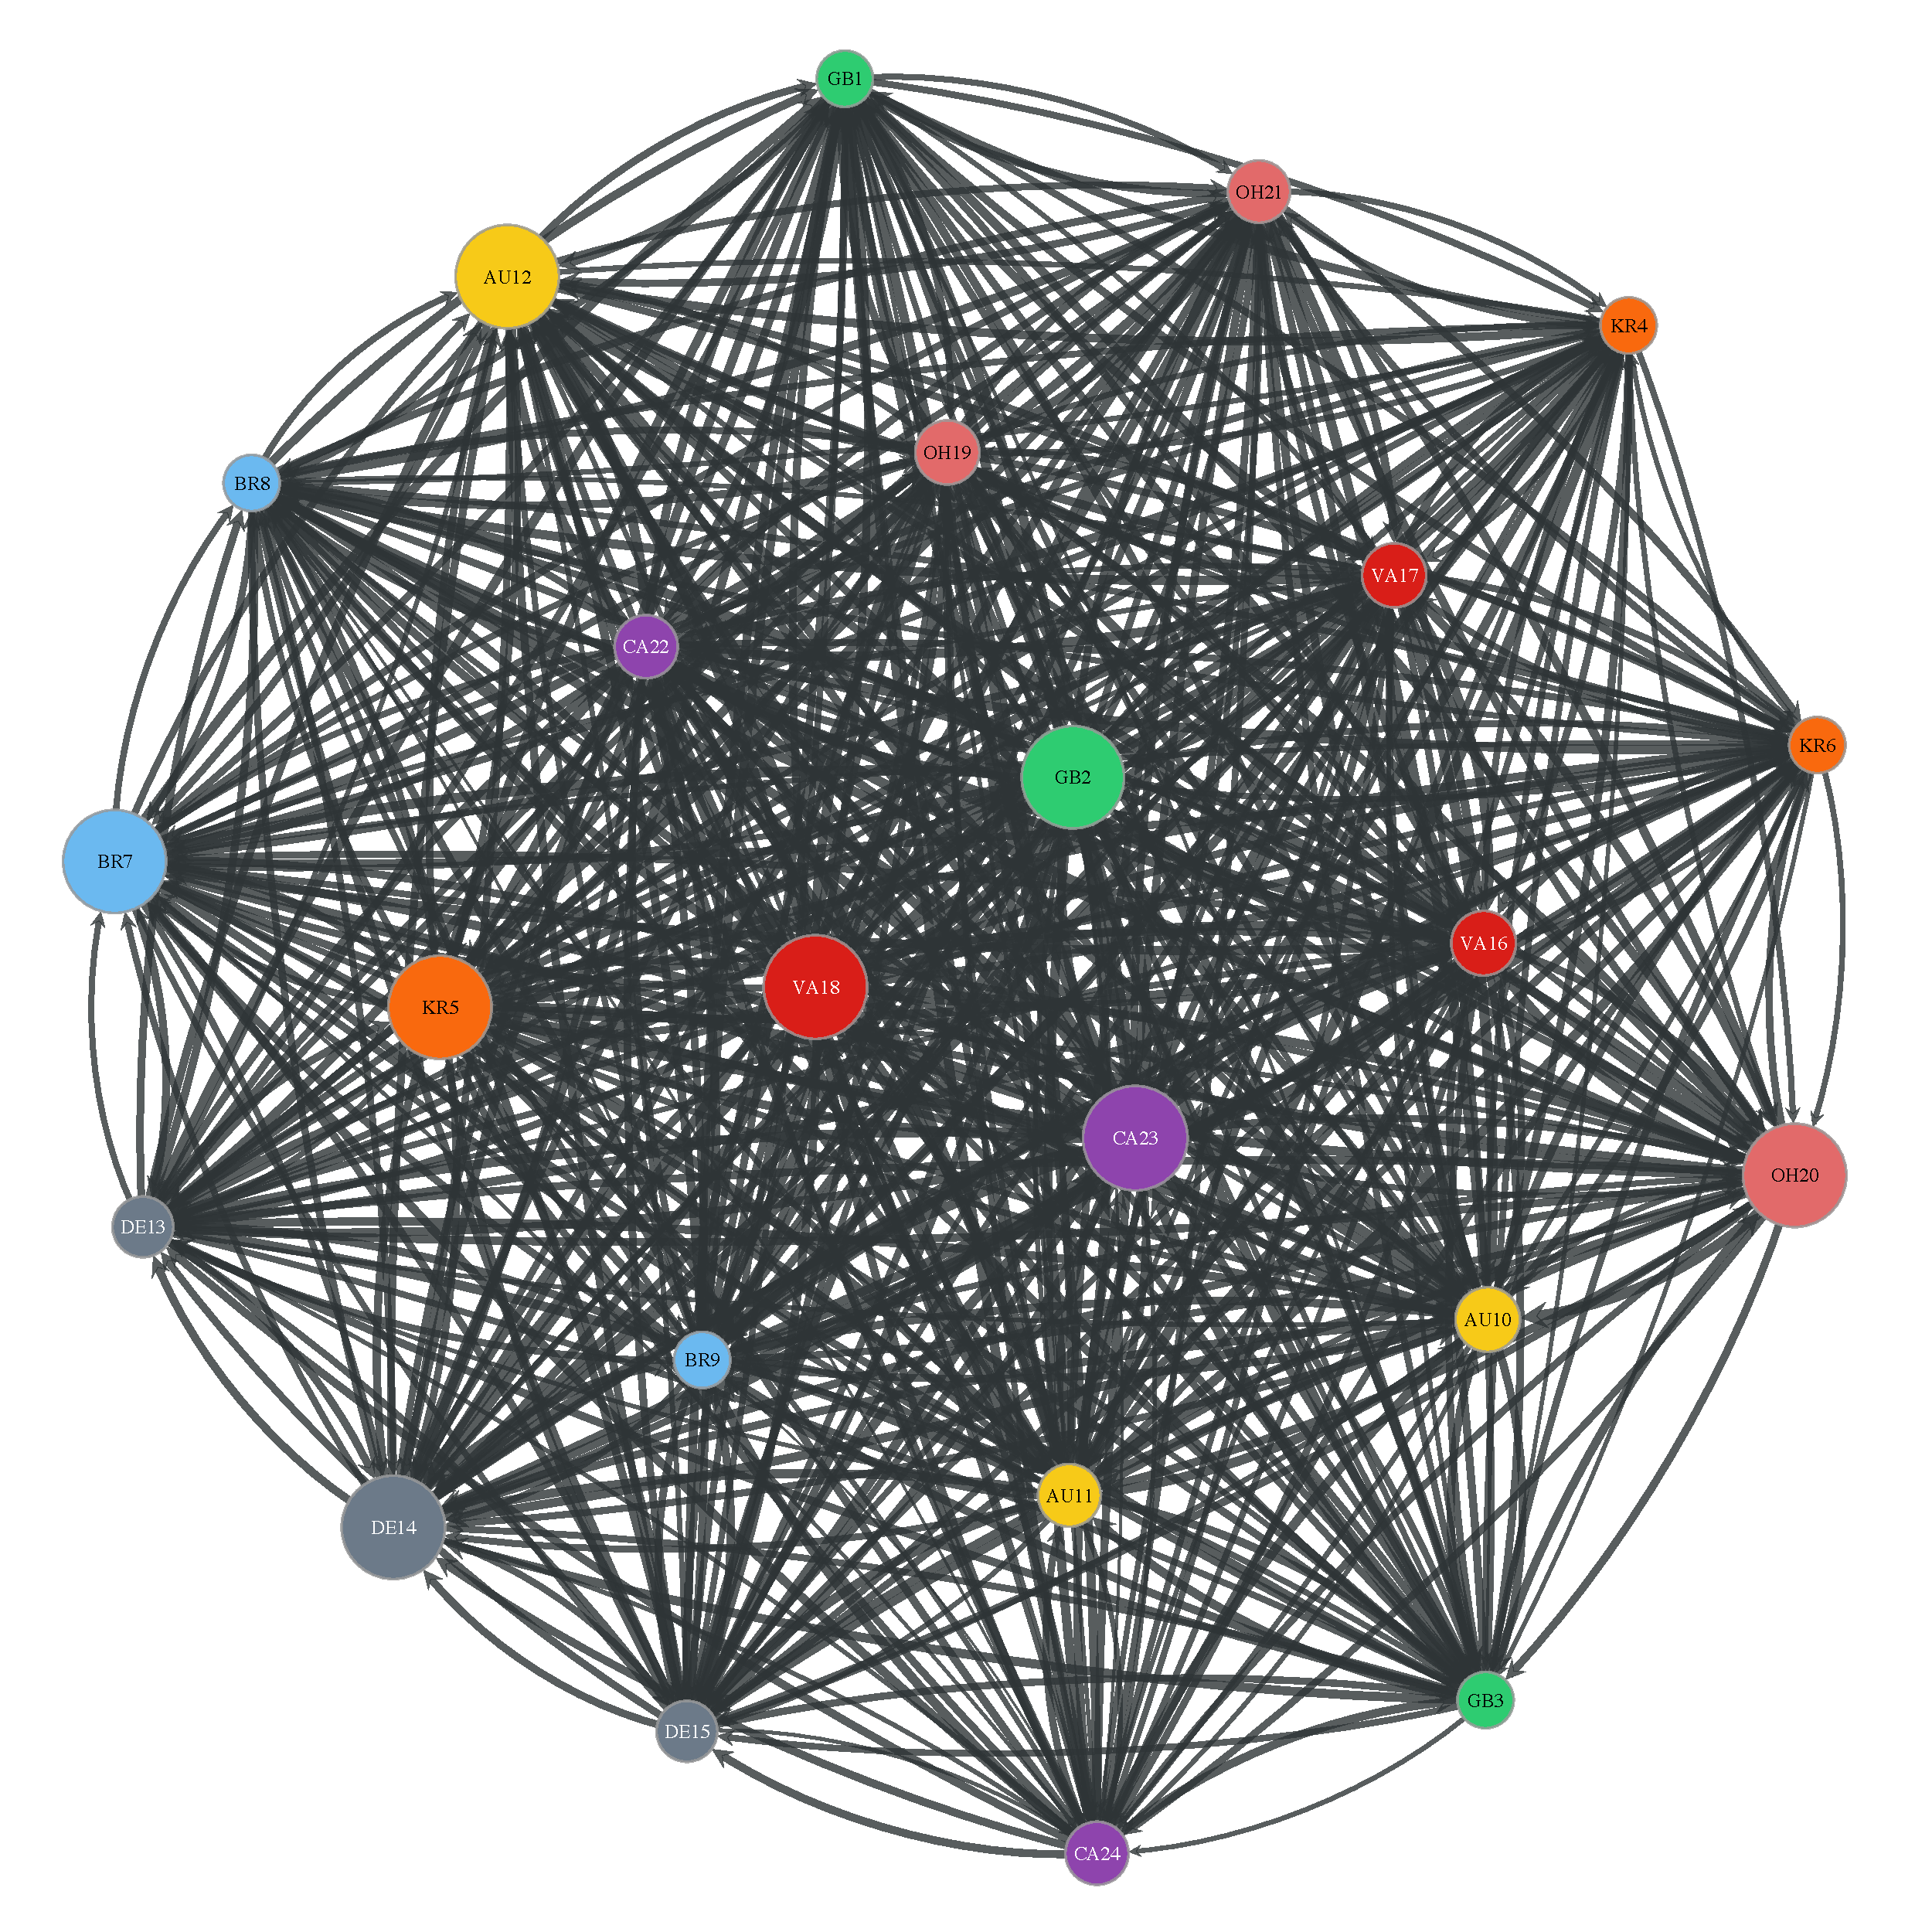
\includegraphics[width=\linewidth]{figures/b-uniform-selection-e1}
      \caption{Uniform Selection}\label{fig:uniform_selection}
    \endminipage\hfill
    \minipage{0.5\textwidth}%
      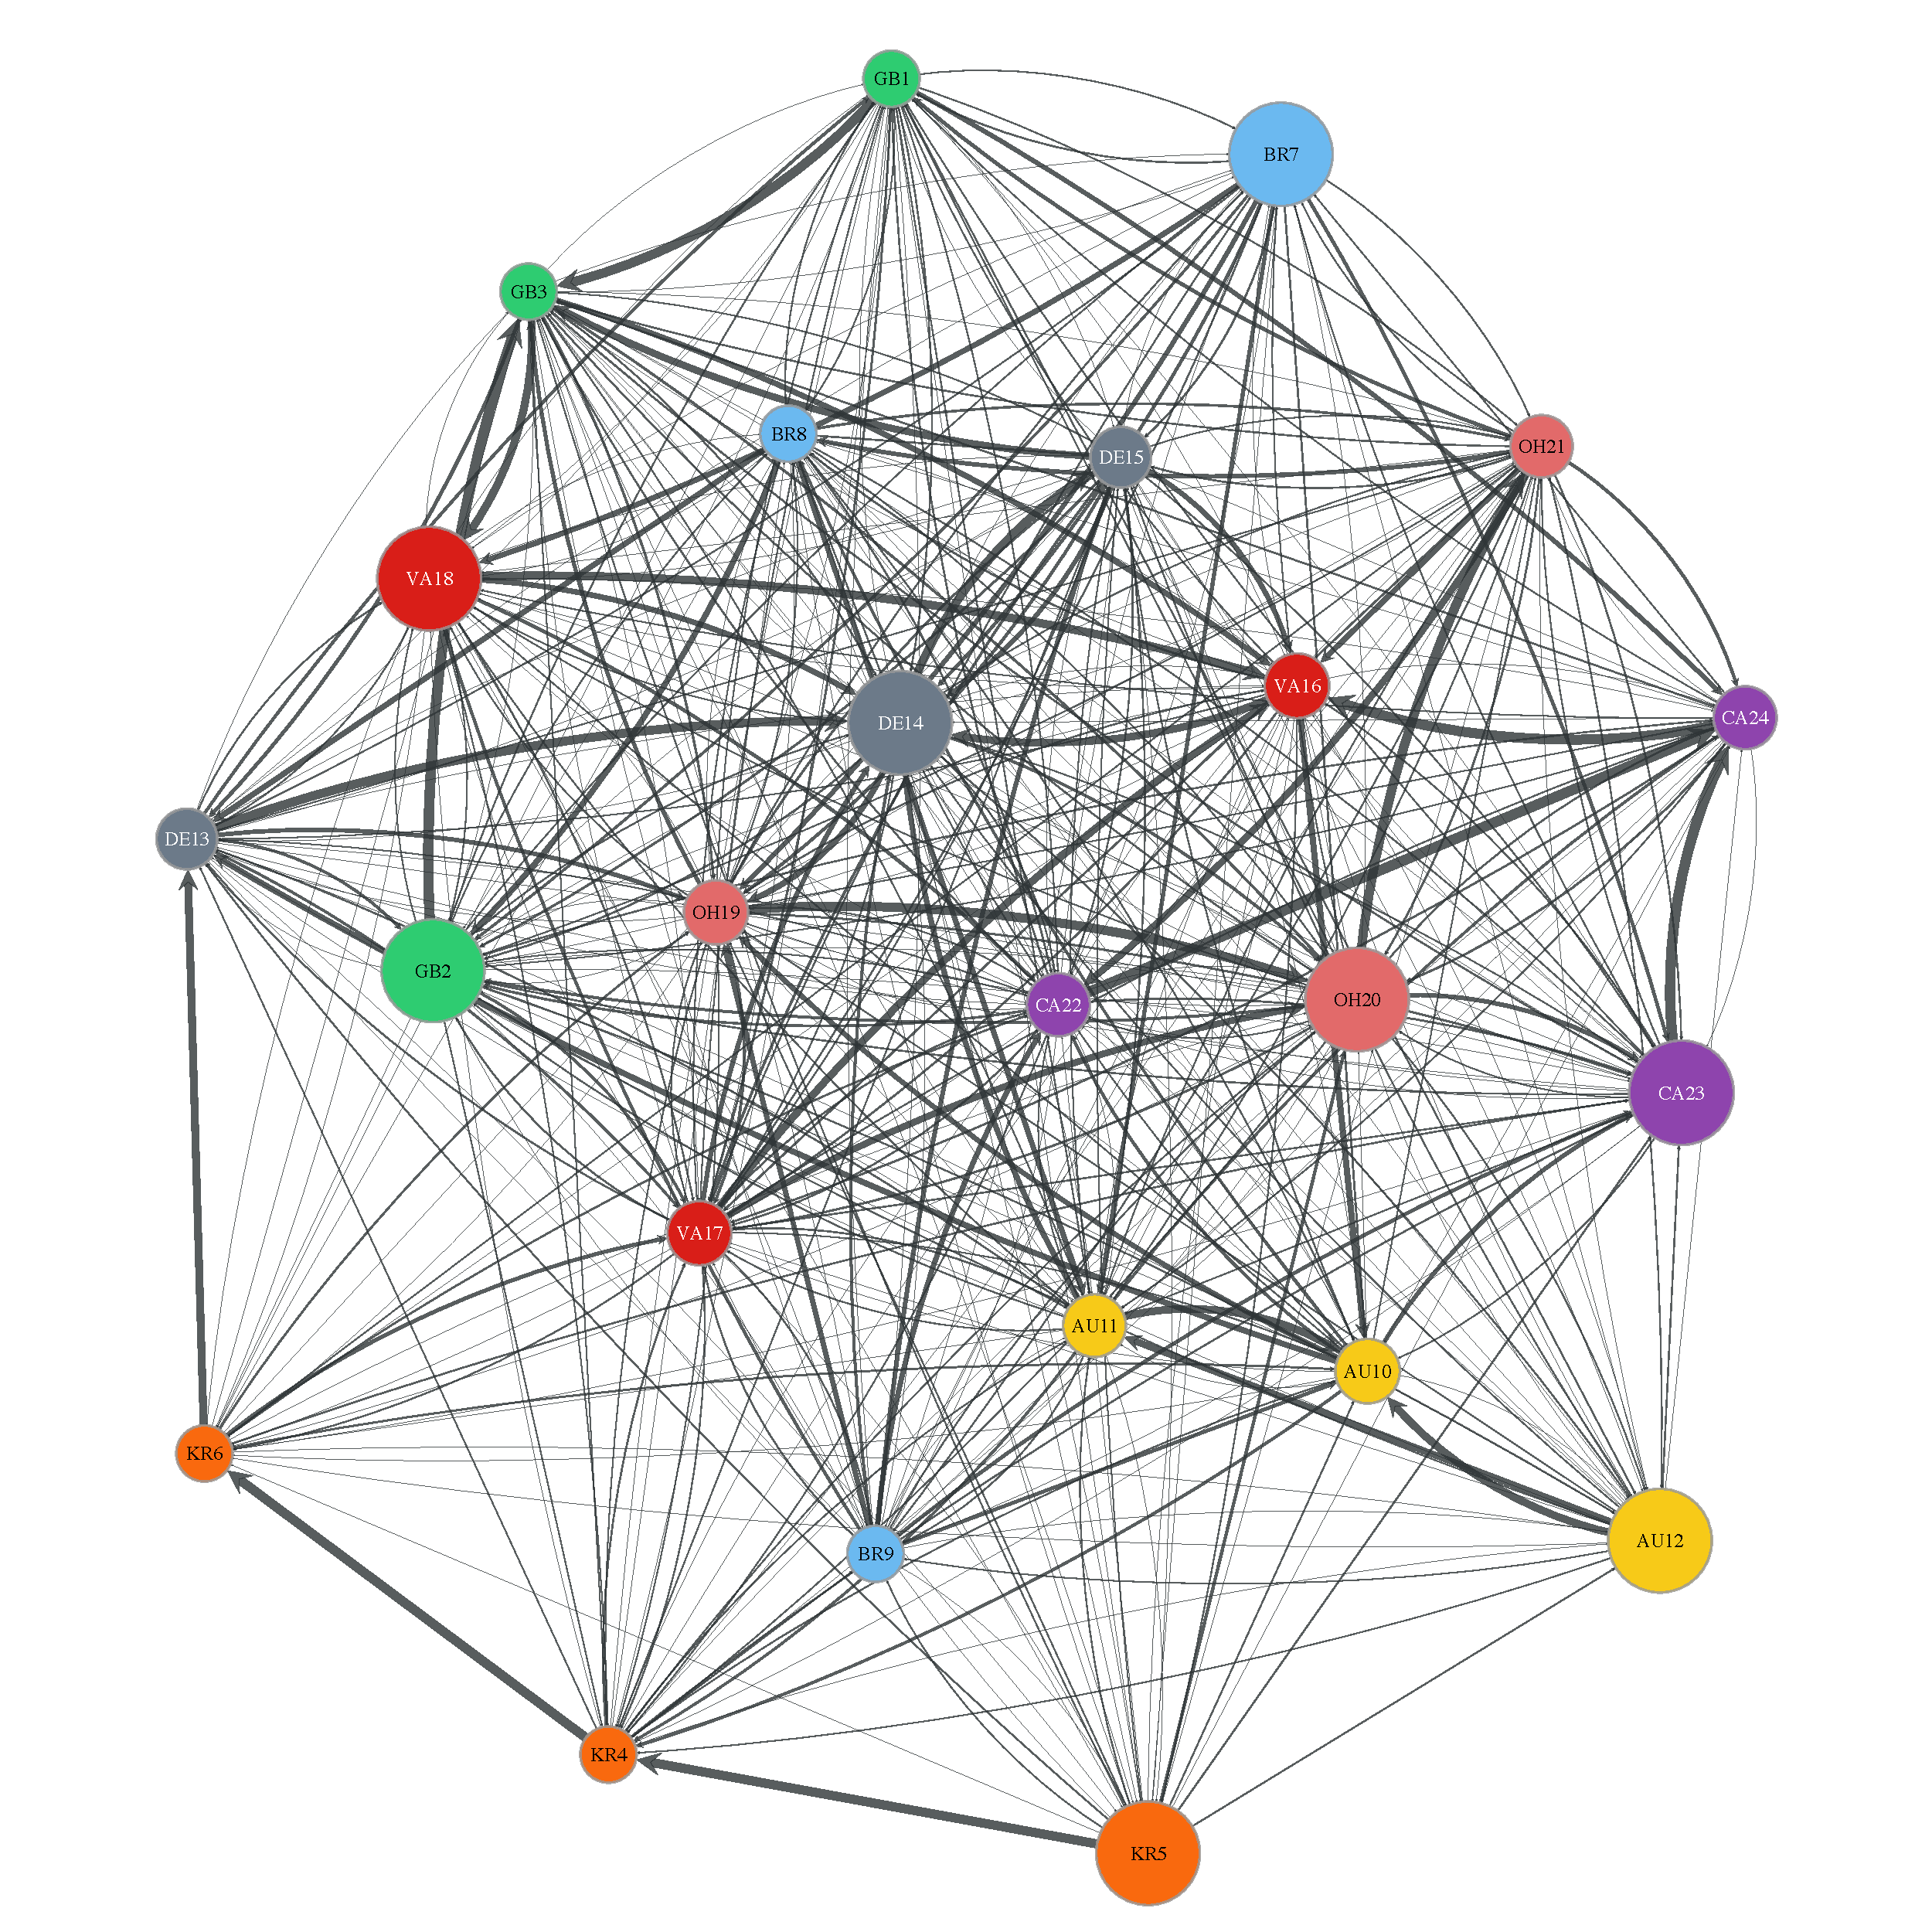
\includegraphics[width=\linewidth]{figures/b-epsilon-greedy-0-1-e2}
      \caption{Epsilon Greedy $\epsilon=0.1$}\label{fig:epsilon_greedy_e1}
    \endminipage
\end{figure*}

\begin{figure*}[t]
    \centering
    \minipage{0.5\textwidth}%
      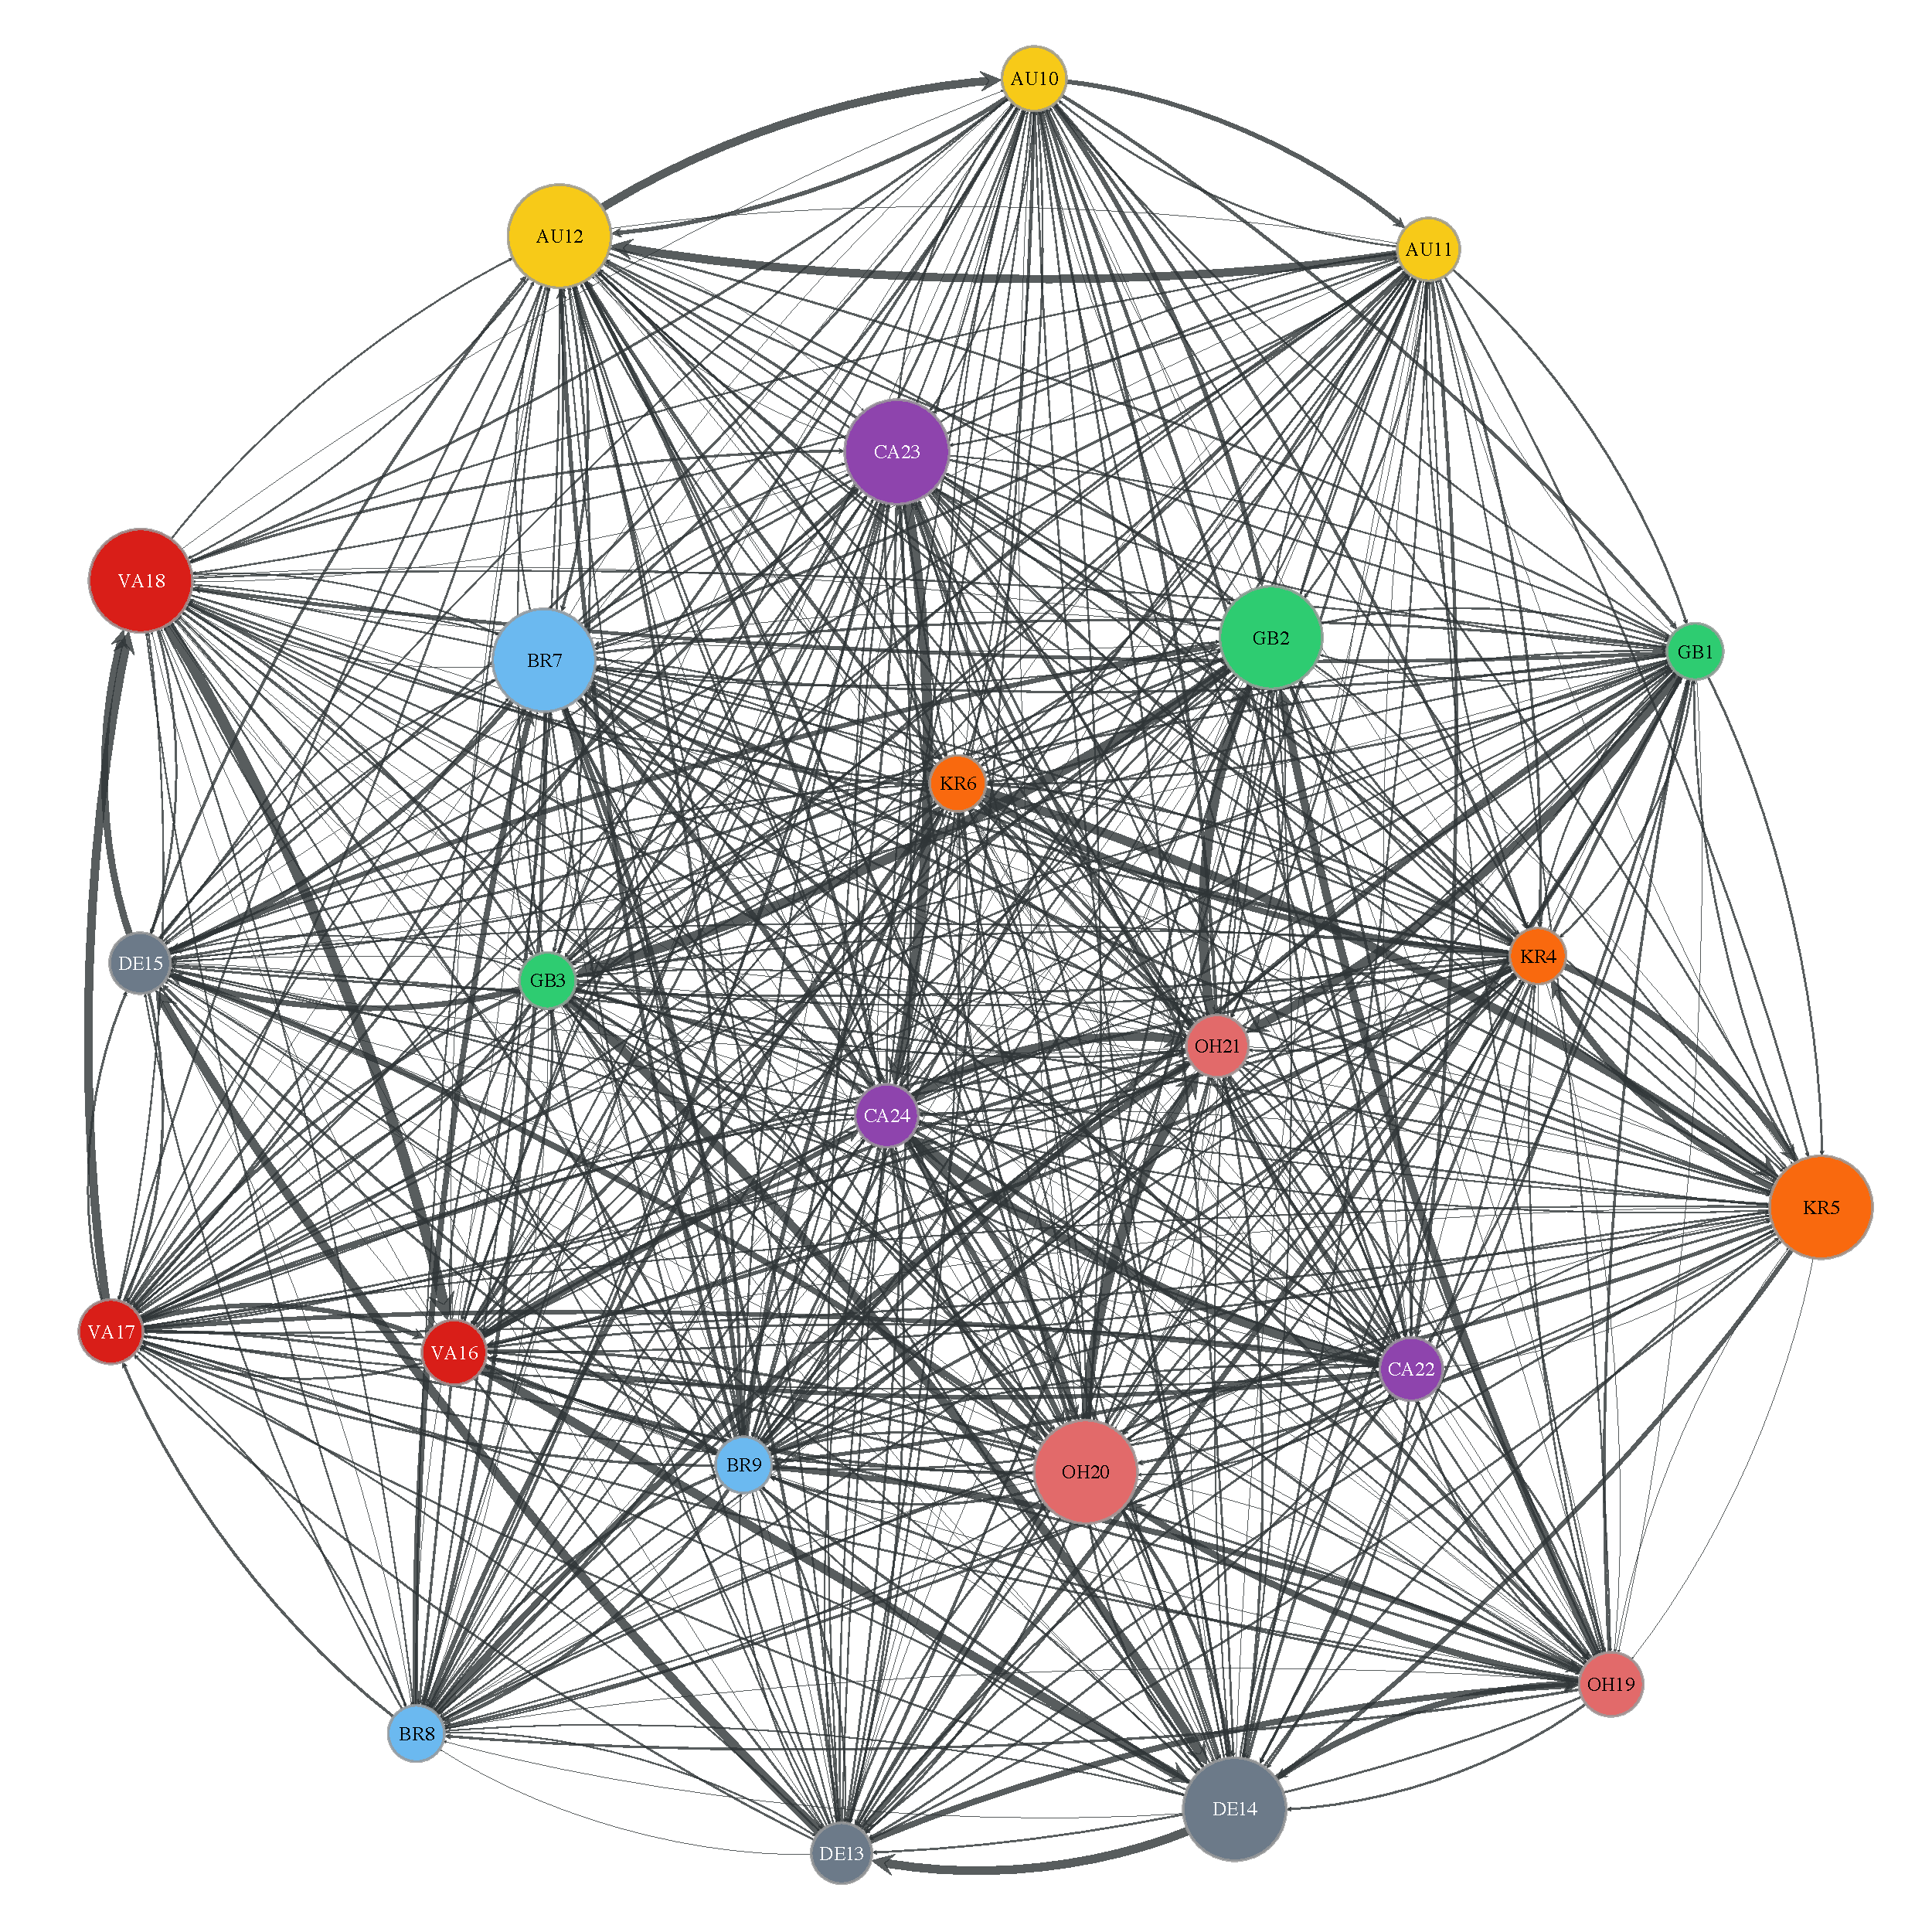
\includegraphics[width=\linewidth]{figures/b-epsilon-greedy-0-2-e3}
      \caption{Epsilon Greedy $\epsilon=0.2$}\label{fig:epsilon_greedy_e2}
  \endminipage\hfill
  \minipage{0.5\textwidth}%
    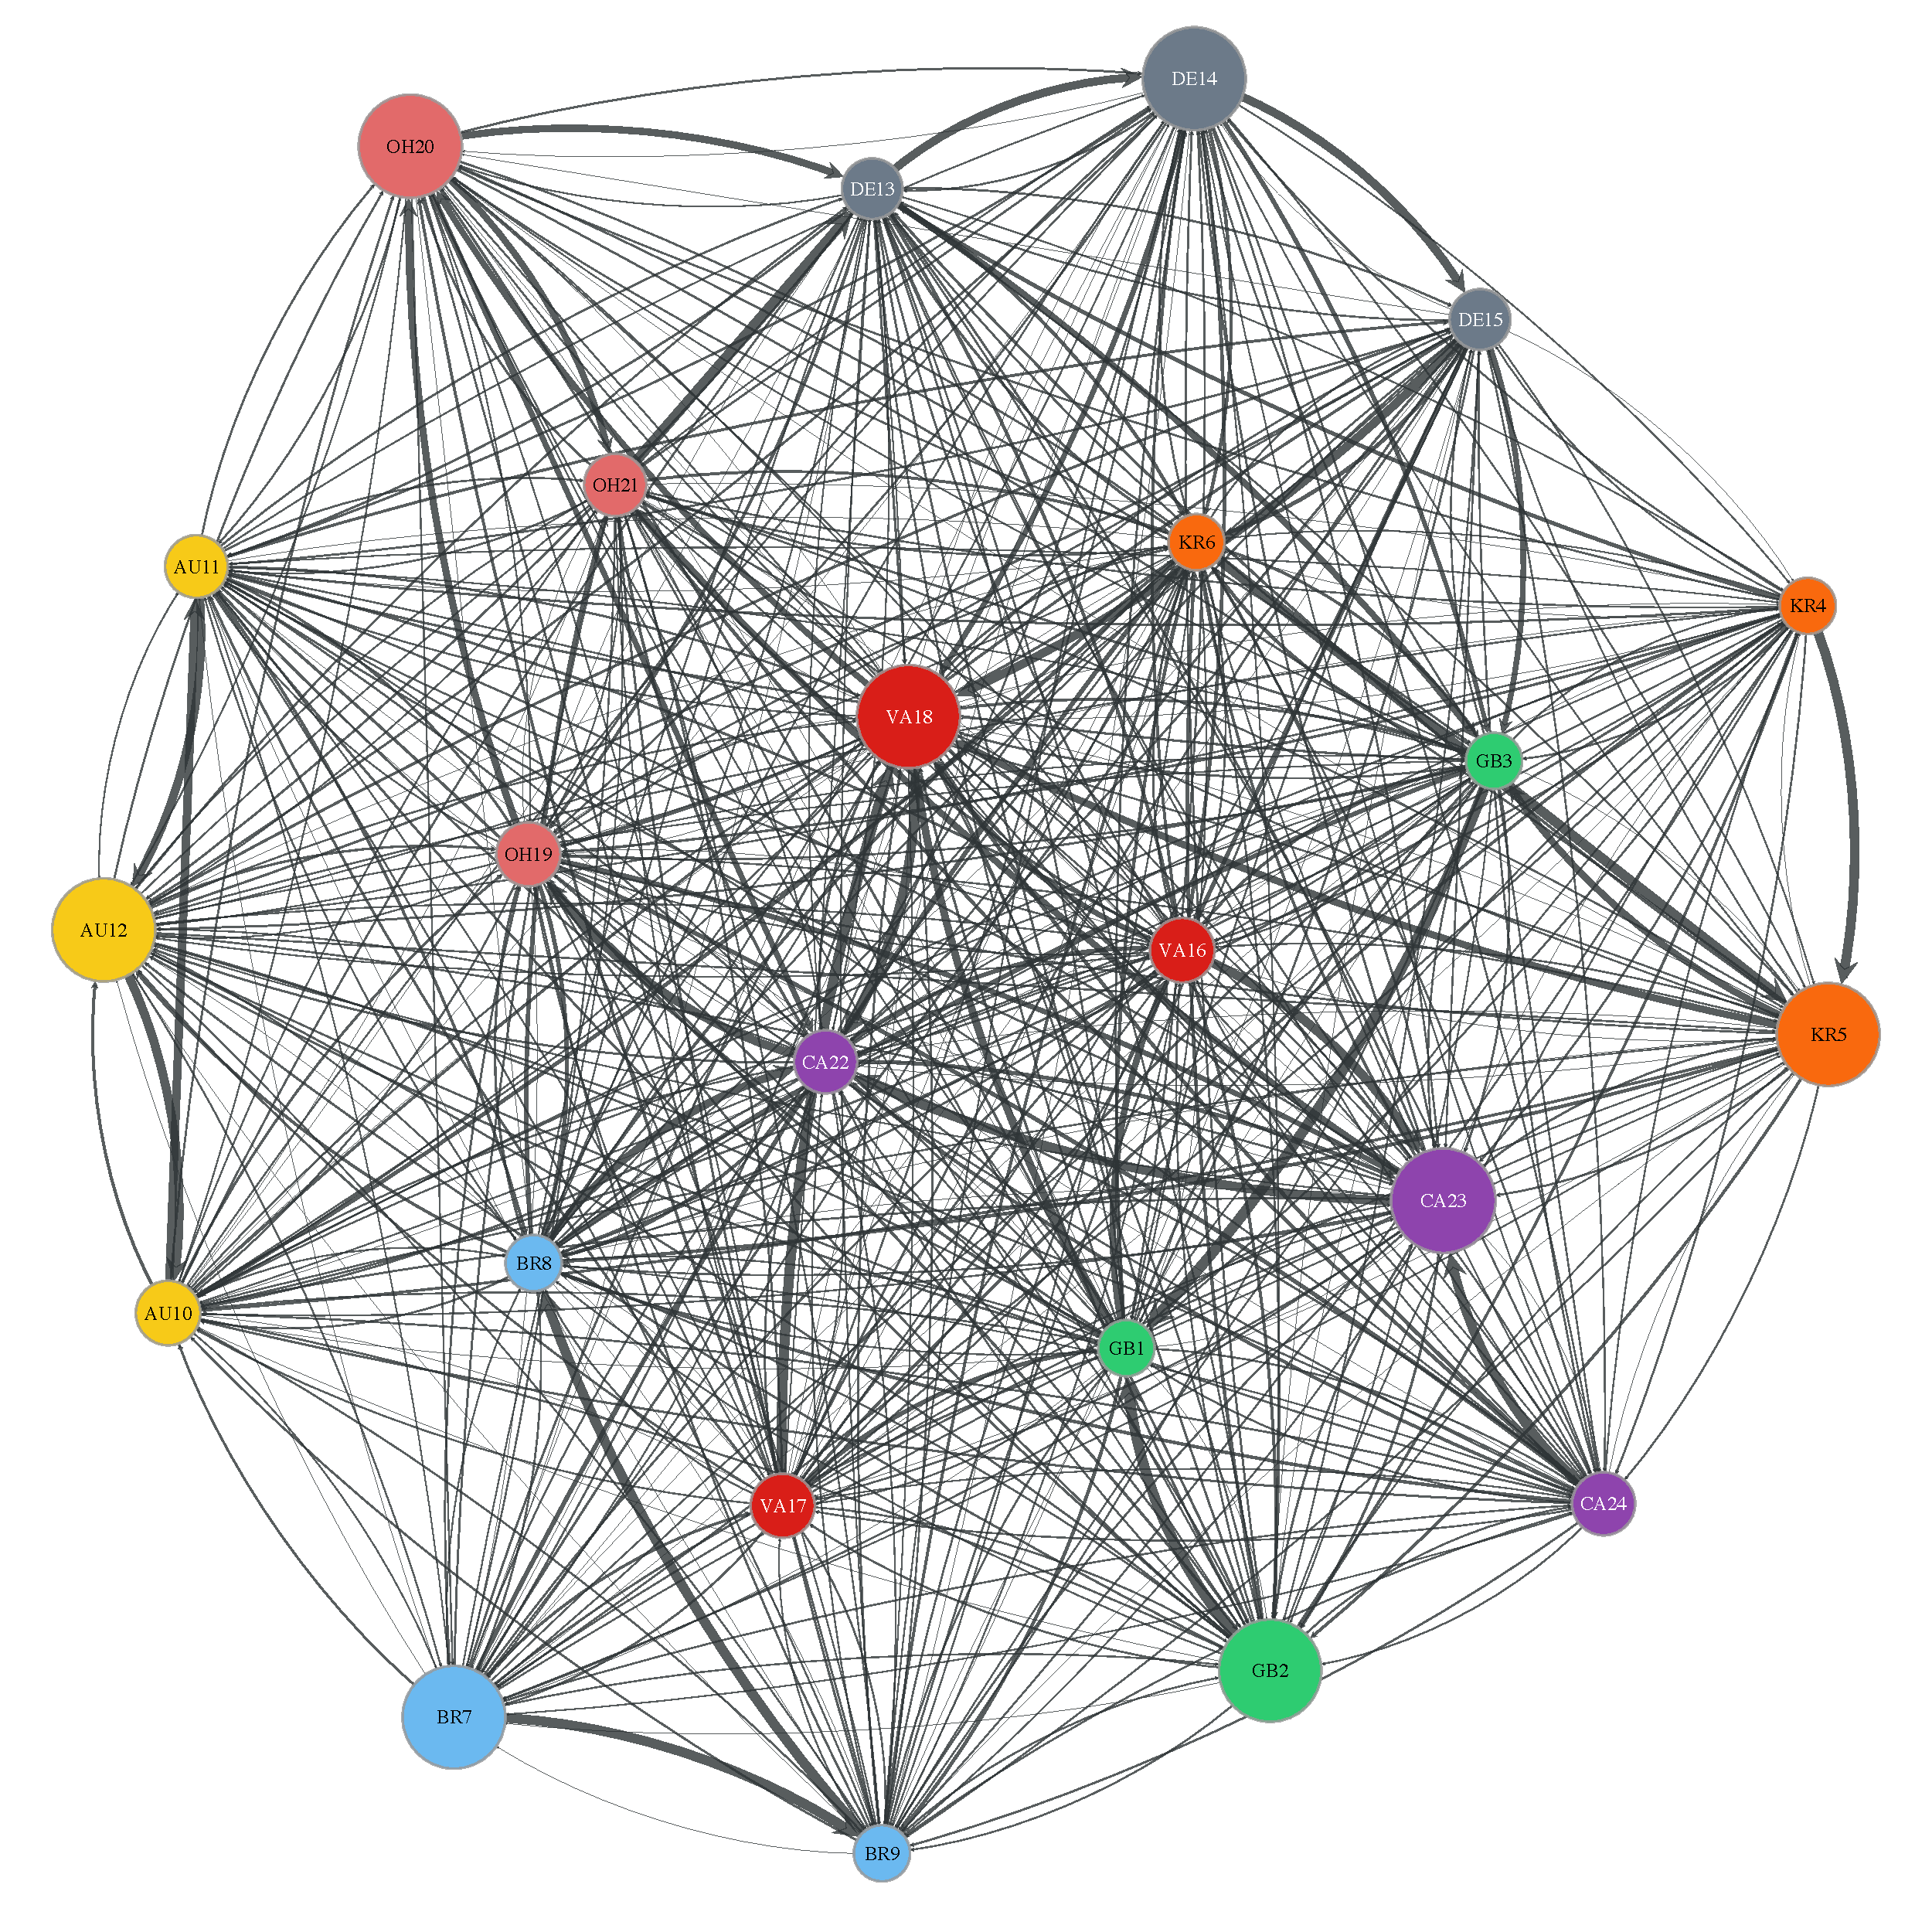
\includegraphics[width=\linewidth]{figures/b-annealing-epsilon-greedy-e5}
    \caption{Annealing Epsilon}\label{fig:annealing_epsilon}
  \endminipage
\end{figure*}


\begin{figure}[t]
    \centering
    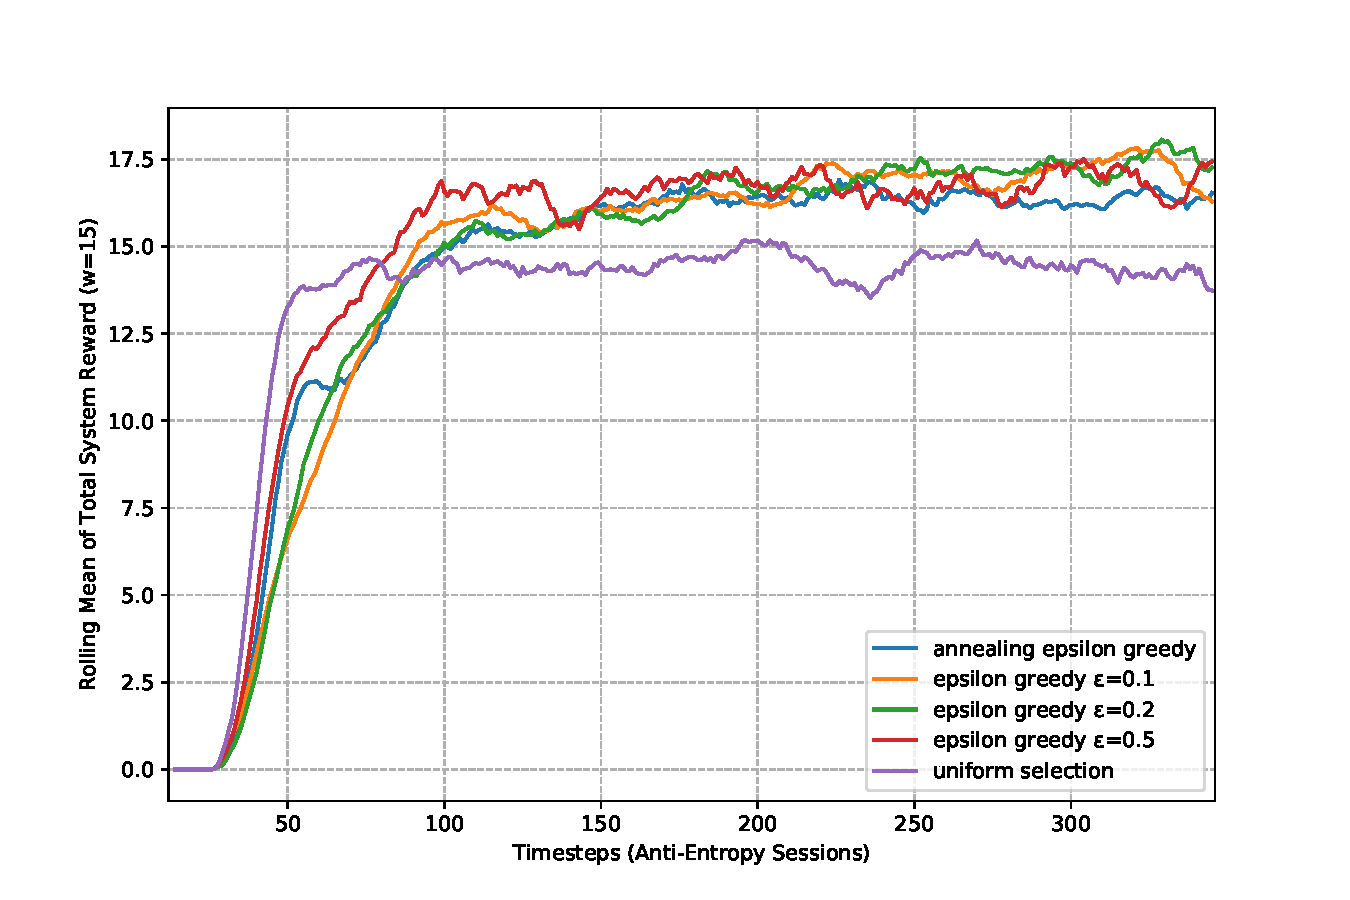
\includegraphics[width=0.5\textwidth]{figures/rewards}
    \caption{Total system rewards over time}
    \label{fig:system_rewards}
\end{figure}

\section*{Discussion}

\section*{Conclusion}

% \begin{acks}
% The authors would like to thank the servers for working so hard.
% \end{acks}
